\section{DeepSmith}

DeepSmith\footnote{DeepSmith available at: \emph{[URL redacted for double-blind review]}} is our open source framework for compiler fuzzing. Figure~\ref{fig:deeptune} provides a high-level overview. In this work we target OpenCL, though the approach is language agnostic. This section describes the three key components: a generative model for random programs, a test harness, and voting heuristics for differential testing.

\begin{figure}
  \centering
  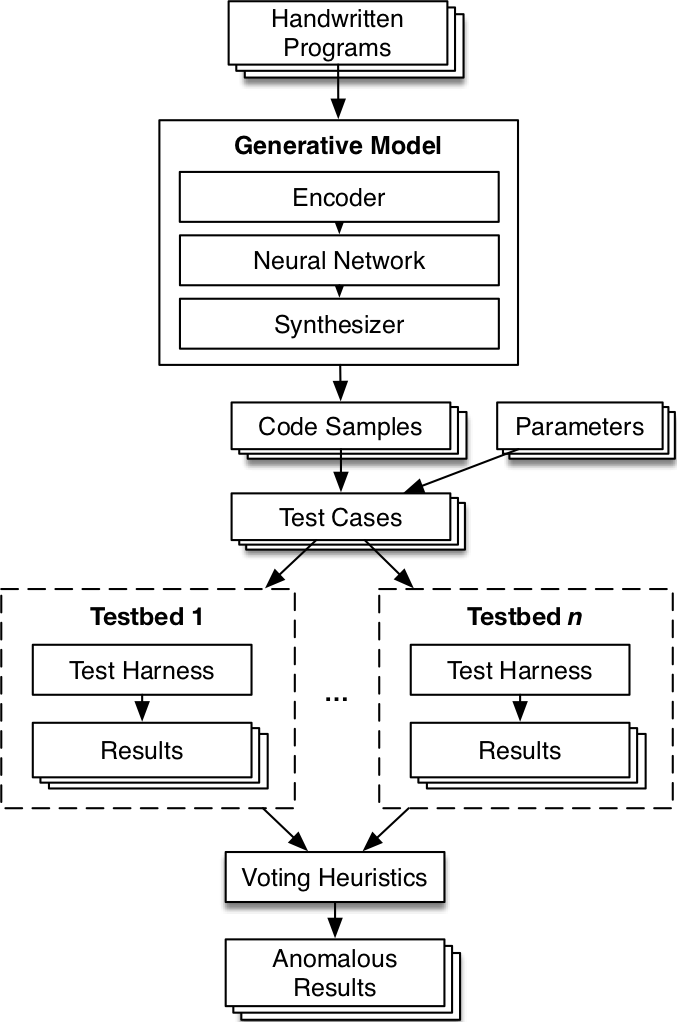
\includegraphics[width=.75\columnwidth]{img/deepsmith} %
  % \vspace{-2em}%
  \caption{%
    DeepSmith system overview.
    \vspace{-1.1em}
  }%
  \label{fig:deeptune}
\end{figure}

\subsection{Generative Model}

Generating test cases for compilers is hard because their inputs are highly structured. Producing text with the right structure requires expert knowledge and a significant engineering effort, which has to be repeated from scratch for each new language. Instead, we treat the problem as an unsupervised machine learning task, employing state-of-the-art deep learning techniques to build models for how humans write programs. Our approach is inspired by breakthrough results in modeling challenging and high dimensional datasets through unsupervised learning~\cite{Raghu2016,Radford2016b,Bowman2015}. Contrary to existing tools, our approach does not require expert knowledge of the target language and is only a few hundred lines of code.

% Contrary to existing tools, this approach is language agnostic, is only a few hundred lines of code, and requires little effort to design.

\paragraph{Handwritten Programs} The generative model needs to be trained on a \emph{seed corpus} of example programs. We automated the assembly of this corpus by mining 10k OpenCL kernels from open source repositories on GitHub. We used an \emph{oracle compiler} (LLVM 3.9) to statically check the source files, discarding files that are not well-formed. The main purpose of this step is to remove the need to manually check that each file selected from GitHub does indeed contain OpenCL. A downside is that any training candidate which triggers a bug in the LLVM 3.9's front end will not be included. However, this did not prevent our system from uncovering errors in that compiler (Section~\ref{subsec:clangs}).

This corpus, exceeding one million lines of code, is used as a representative sample of OpenCL code from which a generative model can be derived.

\paragraph{Encoder} The textual representation of program codes must be encoded as numeric sequences for feeding as input to the machine learning model. Prior machine learning works have used character-level encodings, token-level encodings, or fixed length feature vectors. We extend the hybrid character/token-level encoding of~\cite{Cummins2017b}, in which a programming language's keywords and common names are treated as individual tokens while the rest of the text is encoded on a character-level basis. This approach hits a balance between compressing the input text and keeping the number of tokens in the vocabulary low.

We additionally employed semantic-preserving transformations to simplify the training programs. First, each source file is preprocessed to expand macros and remove conditional compilation and comments. Then, all user-declared identifiers are renamed using an arbitrary, but consistent pattern based on their order of declaration: $\{a,\allowbreak b,\allowbreak c,\allowbreak \ldots,\allowbreak aa,\allowbreak ab,\allowbreak ac,\allowbreak \ldots\}$ for variables and $\{A,\allowbreak B,\allowbreak C,\allowbreak \ldots,\allowbreak AA,\allowbreak AB,\allowbreak AC,\allowbreak \ldots\}$ for functions. This ensures a consistent naming convention, without modifying program behavior. Finally, a uniform code style is enforced to ensure consistent use of braces, parentheses, and white space. These rewriting simplifications give more opportunities for the model to learn the structure and deeper aspects of the language and speed up the learning. On the other hand, some bugs in the preprocessor or front-end might no longer be discoverable. We reason that this is an acceptable trade-off. For languages where the corpus can be many orders of magnitude larger, for example, C or Java, models may be generated without these modifications.

\paragraph{Neural Network} We use the Long Short-Term Memory (LSTM) architecture of Recurrent Neural Network to model program code~\cite{Hochreiter1997}. In the LSTM architecture activations are learned with respect not just to their current inputs but to previous inputs in a sequence. In our case, this allows modeling the probability of a token appearing in the text given a history of previously seen tokens. Unlike previous recurrent networks, LSTMs employ a \emph{forget gate} with a linear activation function, allowing them to avoid the \emph{vanishing gradients} problem~\cite{Pacanu2013}. This makes them effective at learning complex relationships over long sequences~\cite{Lipton2015} which is important for modeling program code. Our LSTM networks model the vocabulary distribution over the encoded corpus. We selected network parameters based on prior works in other domains~\cite{Vinyals,Karpathy2016,Jozefowicz2016a} --- a two layer LSTM network of 512 nodes each, trained using Stochastic Gradient Descent for 50 epochs, with an initial learning rate of 0.002 and decaying by a factor of a half every 5 epochs.

Training the model on the OpenCL corpus took 12 hours using a single NVIDIA Tesla P40. We provided the model with no prior knowledge of the structure or syntax of a programming language.

%Unlike previous recurrent networks in which the strength of learning decreases over time (a symptom of the \emph{vanishing gradients} problem~\cite{Pacanu2013}), LSTMs employ a \emph{forget gate} with a linear activation function, allowing them to retain activations for arbitrary durations. This makes them effective at learning complex relationships over long sequences~\cite{Lipton2015}, an especially important capability for modeling program code, as dependencies in sequences frequently occur over long ranges (for example, a variable may be declared as an argument to a function and used throughout). LSTM networks model the vocabulary distribution over the encoded corpus. We use a two layer LSTM network of 512 nodes each, trained using Stochastic Gradient Descent for 50 epochs, with an initial learning rate of 0.002 and decaying by a factor of a half every 5 epochs. % We use TensorFlow to implement the LSTM networks, with the entire generative model requiring less than 200 lines of Python, and is not specialized to OpenCL.

\paragraph{Program Generation} The trained network is sampled to generate new programs. The model is seeded with the start of a kernel (identified in OpenCL using the keywords \texttt{kernel void}), and sampled token-by-token. A ``bracket depth'' counter is incremented or decremented upon production of \texttt{\{} or \texttt{\}} tokens respectively, so that the end of the kernel can be detected and sampling halted. The generated sequence of tokens is then decoded back to text and used for compiler testing.


\subsection{Test Harness\label{sec:test-harness}}

OpenCL is an embedded compute kernel language, requiring host code to compile, execute, and transfer data between the host and device. For the purpose of compiler fuzzing, this requires a \emph{test harness} to run the generated OpenCL programs. At first, we used the test harness of CLSmith. The harness assumes a kernel with no input and a \texttt{ulong} buffer as its single argument where the result is written. Only 0.2\% of the GitHub kernels share this structure. We desired a more flexible harness so as to test a more expressive range of programs, capable of supporting multi-argument kernels and generating data to use as inputs.

We developed a harness which first determines the expected arguments from the function prototype and generates host data for them. At the moment, we support scalars and arrays of all OpenCL primitive and vector types. For a kernel execution across $n$ threads, buffers of size $n$ are allocated for pointer arguments and populated with values {$[1 \ldots n]$}; scalar inputs are given value $n$, since we observe that most kernels use these for specifying buffer sizes.

The training programs from which the generative model is created are real programs, and as such do not share the argument type restrictions. The model, therefore, may generate correct programs for which our driver cannot create example inputs. In this case, a ``compile-only'' stub is used, which only compiles the kernel, without generating input data or executing the compiled kernel.

Unlike the generative model, this test harness is language-specific and the design stems from domain knowledge. Still, it is a relatively simple procedure, consisting of a few hundred lines of Python.

%OpenCL kernels are executed concurrently one or more threads. We parameterize test harness generation with a single value $n$. For each program, we generate two test harnesses, one where $n=1$ (i.e. a single thread computing a single result) and one where $n = 2048$. For a given OpenCL kernel, we first parse the function prototype in order to determine the expected arguments. We then generate host data to feed to these arguments --- supporting scalars and arrays of all OpenCL primitive and vector types. Buffers of size $n$ are allocated for pointer arguments, and populated with values {$[1 \ldots n]$}; scalar inputs are given value $n$. We then enqueue the kernel on $n$ threads. The \emph{output} of a program is the values of all non-const arguments after kernel execution.

%Since we do not guarantee that the generative model samples are well-formed, it may not be possible to parse the function signature. In this case, a ``compile-only'' stub is generated, which only compile the kernel, without generating input data or executing the compiled kernel.

%We note that, unlike the generative model, this test harness is language-specific and the design from stems domain knowledge. Still, it is a relatively simple procedure, consisting of a few hundred lines of Python.

% SELECT (SUM(compile_only) / (
% SELECT COUNT(*)
% FROM CLgenResults results
% INNER JOIN CLgenMetas meta ON results.id = meta.id
% WHERE cumtime < 48 * 3600
% )) * 100 as '% compile-only'
% FROM CLgenResults results
% INNER JOIN CLgenMetas meta ON results.id = meta.id
% INNER JOIN CLgenHarnesses harnesses on results.testcase_id = harnesses.id
% WHERE cumtime < 48 * 3600;
% 21.5\% of test cases are compile-only stubs.


% We classify the result of executing a test case into one of six classifications: build failure (\abf), build crash (\bc), runtime crash (\arc), or pass (\textbf{\cmark}). A \abf occurs when compilation of a kernel fails, usually accompanied by an error message. A \bc outcome occurs when the compiler crashes. A \arc outcome occurs when the program crashes during execution. The \bto and \textbf{to} outcomes occur when the program compilation or execution time out, respectively.

\paragraph*{Test Harness Output Classes}
\begin{figure}
  \centering %
  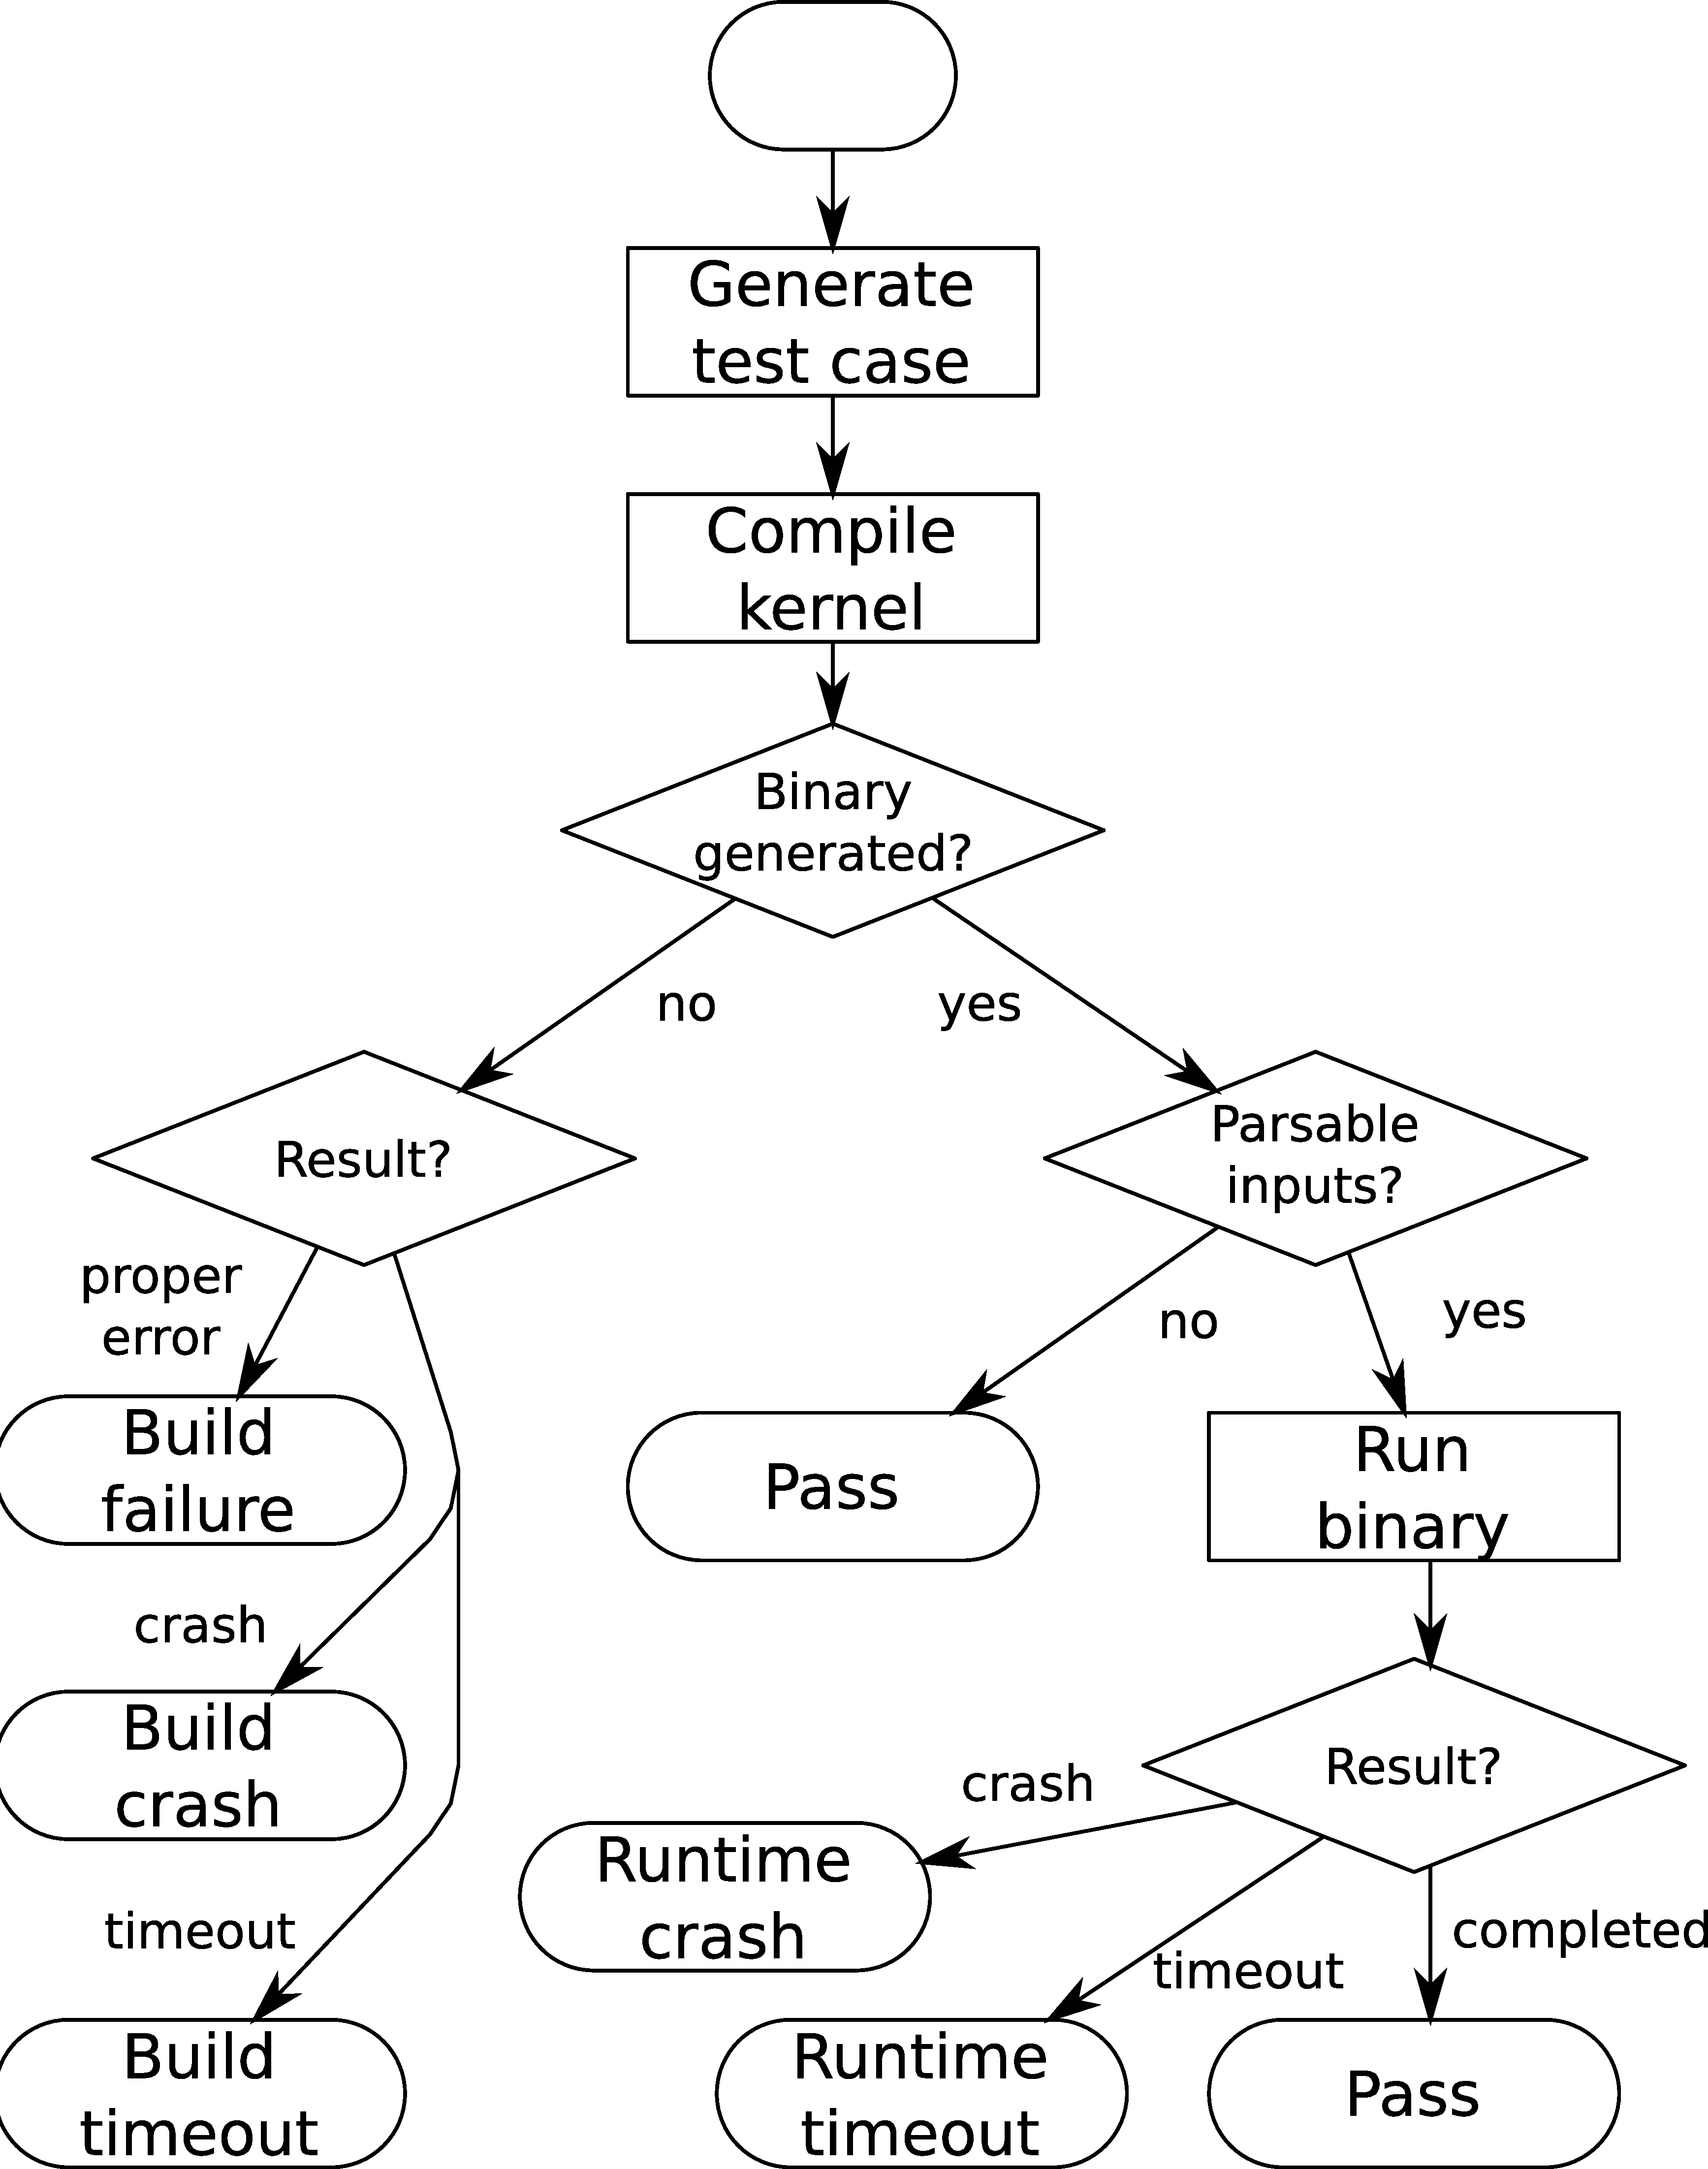
\includegraphics[width=.8\columnwidth]{img/testprocess-long}%
  \caption{%
 	  Test case execution, and possible results.%
     \vspace{-1.1em}
  }%
  \label{fig:test-process} %
\end{figure}
Executing a test case on a testbed leads to one of seven possible outcomes, illustrated in Figure~\ref{fig:test-process}.
A \emph{build failure} occurs when online compilation of the OpenCL kernel fails, usually accompanied by an error diagnostic.
A \emph{build crash} or \emph{build timeout} outcome occurs if the compiler crashes or fails to produce a binary within 60 seconds, respectively.
For compile-only test cases, a \emph{pass} is achieved if the compiler produces a binary.
For test cases in which the kernel is executed, kernel execution leads to one of three potential outcomes:
\emph{runtime crash} if the program crashes,
\emph{timeout} if the kernel fails to terminate within 60 seconds,
or \emph{pass} if the kernel terminates gracefully and computes an output.

\subsection{Voting Heuristics for Differential Testing}

We employ established Differential Testing methodologies to expose compiler defects. As in prior work, voting on the output of programs across compilers has been used to circumvent the \emph{oracle problem} and detect miscompilations~\cite{McKeeman1998}. However, we extend this approach to describe not only miscompilations, but also anomalous build failures and crashes.


%
%\begin{enumerate}
%	\item \emph{Build failure} (\abf) Online compilation of the OpenCL kernel fails, usually accompanied by an error diagnostic.
%	\item \emph{Build crash} (\bc) The compiler crashes during online compilation of the OpenCL kernel.
%	\item \emph{Build timeout} (\bto) Online compilation of the OpenCL kernel exceeds the timeout of 60 seconds.
%	\item \emph{Runtime crash} (\arc) Compilation of the OpenCL kernel succeeds gracefully, but the program crashes during kernel execution.
%	\item \emph{Runtime timeout} (\textbf{to}) Compilation of the OpenCL kernel succeeds gracefully, but program execution exceeds the timeout of 60 second.
%	\item \textbf{\cmark} \emph{Completion} The program terminates gracefully and produces an output.
%\end{enumerate}

\begin{table*}[t!]
	\footnotesize %
	\centering %
	% \rowcolors{2}{white}{gray!25}
	\begin{tabular}{rlllllllrr}
\toprule
 \#. &                                             Device &              Platform &    Driver & OpenCL &      Operating system &  Device type & Testing time &  B.R. Generated &  B.R. Submitted \\
\midrule
  1 &                                   GeForce GTX 1080 &           NVIDIA CUDA &    375.39 &    1.2 &    Ubuntu 16.04 64bit &          GPU &          30h &              13 &               7 \\
  2 &                                    GeForce GTX 780 &           NVIDIA CUDA &    361.42 &    1.2 &  openSUSE  13.1 64bit &          GPU &           0h &               0 &               0 \\
  3 &           Intel(R) HD Graphics Haswell GT2 Desktop &  Intel Gen OCL Driver &       1.3 &    1.2 &    Ubuntu 16.04 64bit &          GPU &           2h &              35 &              11 \\
  4 &          Intel(R) Xeon(R) CPU E5-2620 v4 @ 2.10GHz &          Intel OpenCL &  1.2.0.25 &    2.0 &    Ubuntu 16.04 64bit &          CPU &          10h &              10 &               5 \\
  5 &          Intel(R) Xeon(R) CPU E5-2650 v2 @ 2.60GHz &          Intel OpenCL &  1.2.0.44 &    1.2 &      CentOS 7.1 64bit &          CPU &           7h &               2 &               1 \\
  6 &            Intel(R) Core(TM) i5-4570 CPU @ 3.20GHz &          Intel OpenCL &  1.2.0.25 &    1.2 &    Ubuntu 16.04 64bit &          CPU &           1h &               4 &               4 \\
  7 &    Intel(R) Many Integrated Core Acceleration Card &          Intel OpenCL &       1.2 &    1.2 &      CentOS 7.1 64bit &  Accelerator &          11h &               0 &               0 \\
  8 &  pthread-Intel(R) Xeon(R) CPU E5-2620 v4 @ 2.10GHz &                  POCL &      0.14 &    2.0 &    Ubuntu 16.04 64bit &          CPU &          15h &             170 &              52 \\
  9 &                                 Oclgrind Simulator &              Oclgrind &     16.10 &    1.2 &    Ubuntu 16.04 64bit &     Emulator &           9h &               0 &               0 \\
\bottomrule
\end{tabular}

	\caption{%
		OpenCL systems and the number of bug reports submitted to date. For each system, two testbeds are created, one with compiler optimizations, the other without.%
		\vspace{-.5em}
	}
  \vspace{-1.8em}
	\label{tab:platforms}
\end{table*}

When evaluating the outcomes of test cases, build crash (\bc) and build timeout (\bto) outcomes are of immediate interest, indicative of erroneous compiler behavior (examples may be found in Section~\ref{subsec:compile-time-defects}). For all other outcomes, \emph{differential tests} are required to confirm anomalous behavior. We look for test cases where there is a majority outcome -- i.e. for which some fraction of the testbeds behave the same -- but some testbed deviates. We use the presence of the majority increasing the likelihood that there is a `correct' behavior for the test case. In this work, we choose the majority fraction to be $\ceil{\frac{2}{3}n}$, where $n$ is the number of testbeds.

An \emph{anomalous build failure} (\abf) or \emph{anomalous runtime crash} (\arc) occurs if, for a given test case, the majority of testbeds execute successfully, and a testbed yields a compilation error or runtime crash.
An \emph{anomalous wrong-output} (\awo) occurs if, for a given test case, the majority of testbeds execute successfully, producing the same output values, and a testbed yields a result which differs from this majority output. Anomalous wrong-output results are indicative of \emph{miscompilations}, a particularly hard to detect class of bug in which the compiler silently emits wrong code. CSmith is designed specifically to target this class of bug.

% Only 2.3\% of CLSmith programs with anomalous outputs are insensitive to optimization level.

%
%\begin{enumerate}
%	\item \awo \emph{Wrong code} Program terminates gracefully, but computes a result which differs from the majority output. For a DeepSmith result to be classified with \emph{wrong-code}, we require first that the program passes verification using GPUVerify~\cite{Betts2012}, and that a reference run with Oclgrind~\cite{Price2015} produces no warnings. \cc{Vote on compiler warnings, and optimization sensitivity. This means we way miss bugs which optimization level insensitive, though our experiences testing with CLSmith revealed only discovered 2 such cases}.
%	\item \abf \emph{Build failure} Online compilation of OpenCL program fails, whereas the majority of testbeds produce a binary. \cc{TODO: with voting to exclude programs which rely on OpenCL 2.0 / compiler specific features}
%	\item \arc \emph{Runtime crash} One or more OpenCL API calls return an error status during the program execution, or the program crashes.
%	\item \textbf{to} \emph{Runtime timeout} Program execution exceeds the timeout of 60 second, whereas the majority of testbeds produce an output.
%\end{enumerate}


% \subsection{Design Trade-Offs}\label{subsec:discussions}
% Discussions?


% \paragraph{Design Trade-Offs}
%Our sequence-to-sequence approach to program generation greatly simplifies the implementation --- targeting a new language requires only a corpus of example programs and a test harness for generated codes. The generative model itself contains no language-specific code, and is implemented in less than 200 lines of Python --- a small fraction of that of prior approaches. The trade-off of this makes significantly reduces the cost of development, but we provide no guarantees on generated program correctness. \cc{not well formed, not well typed, and not free from undefined behavior}

\paragraph{False Positives for Anomalous Runtime Behavior}\label{subsec:discussions}
Generated programs may contain undefined or non-deterministic behavior which will incorrectly be labeled as anomalous. CSmith circumvents this problem by performing  complex analyses during generation so as to minimize the chance of producing programs with undefined behavior. Although similar analyses could be created as filters for our system, we take a simpler approach, filtering only the few types of non-deterministic behavior we have actually observed to happen in practice.

We filter data races, out-of-bounds and uninitialized accesses with GPUverify~\cite{Betts2012} and Oclgrind~\cite{Price2015}. Some compiler warnings provide strong indication of non-deterministic behavior (e.g. comparison between pointer and integer) -- we check for these warnings and filter accordingly.

% Vendor support for OpenCL standard versions is inconsistent, as is the support for optional language extensions. Since we do not version the GitHub corpus on which we built the DeepSmith models, we might generate code which uses features not supported by a testbed. Such cases were trivially detectable through compiler error messages which we used to prevent false-positives for anomalous build failures.

Floating point operations in OpenCL can be imprecise, so code can produce different output on different testbeds. For this reason, CSmith and CLSmith do not support floating point operations. DeepSmith allows floating point operations but since it cannot apply differential testing on the outputs, it can detect all results except for the \emph{anomalous wrong-output} results.

The last type of undefined behavior we observed comes from division by zero and related mathematical functions which require non-zero values. We apply a simple detection and filtering heuristic -- we change the input values and check to see if the output remains anomalous. While theoretically insufficient, in practice we found that no false positives remained.

%\paragraph{Undefined Behaviors} % aka. unambiguous observable behaviour
%Differential testing is valid only for programs that do not rely on undefined behavior. Detecting such cases is difficult, especially since OpenCL does not have the rich toolset of C, for example CompCert or UBSan. Some errors such as data races and out-of-bounds accesses can be caught with GPUverify~\cite{Betts2012} and Oclgrind, while compiler warnings may indicate undefined behavior (e.g. comparison between pointer and integer). For the rest, our approach does not rule out manual inspection. DeepSmith programs are short and easily interpretable, so manual inspection is feasible. Still, we have not yet discovered a false-positive result which was not trivially detectable by automated filtering.

%\paragraph{OpenCL Versions and Extensions} OpenCL is a fast evolving language, with six standard revisions in eight years. Vendor support for standard versions is inconsistent, as is the support for optional language extensions. Since we do not version the GitHub corpus on which we built the DeepSmith models, this has the potential to lead to false-positive results for programs which depend upon features which are not supported by a testbed. For example, not all testbeds support the optional \texttt{cl\_khr\_fp64} extension which provides support for double-precision floating point. We found that such results were trivially detectable through compiler error messages, and used to prevent false-positives for anomalous build failures.

%\paragraph{Floating Points} Floating point operations in OpenCL can be imprecise within bounds. Since errors propagate, the same correct code can produce significantly different output on different testbeds. For this reason, CSmith and CLSmith do not support floating point operations. This restriction is artificially limiting, since floating point computations are dominant in the common uses of OpenCL. Instead, we generate, compile, and execute floating point kernels, we just do not subject their outputs to differential testing so we cannot detect a \awo result.
% $ ls | xargs grep -E -l '(float|double)' -- | wc -l  # 2245
% 48\% of GitHub kernels use floating points.



% \paragraph{Divide-by zero} \cc{TODO} The hardest false-positive to prevent was division by zero and related mathematical functions which require non-zero values. In all cases we discovered these can be detected by simply changing the input values and checking to see if the output remains anomalous.

% Section 7.4 of OpenCL 1.2 spec.
% HJL- IMO just bin this
%\cc{Find a home:} Random token / grammar enumeration has previously been used to target parsers and lexers. CSmith creates huge, ``ugly'' programs with the intention of deliberately targeting bugs in IR transformations --- the middle-end.

%One might expect our approach --- generating small test cases in the style of handwritten programs --- is perhaps less likely to find bugs than CSmith, which generates huge, ``ugly'' programs pairing infrequently used language features. DeepSmith rarely generates large OpenCL kernels because humans rarely write them. A code which is more likely to be written by a human is also more likely to be included in the compiler test suites, \cc{hmm what do we do about this}
